\section{Use Case and Model Design} \label{sec:Approach}

Our objective is to build a robust Testbed that behaves like a real urban traffic light control system.
As presented in section \ref{Sec:Related_Works},
	a crossroad traffic light design has been proposed based on PNs \cite{huang_modular_2014}.
Authors demonstrated the necessity to monitor checkpoints like traffic light transitions from red to green and define critical control points to ensure that the transition model is correct.
Authors have identified which signal indication sequence optimizes the overall system performance.
We were inspired from this work by adding the vulnerability of wireless network \emph{i.e.} packet loss.
Indeed,
	this model is theoretical and static,
	and would not model entirely traffic light control system.
Thus,
	we propose a UPPAAL timed automata for modelling and verification of the system.

\subsection{Use case}

We consider the use case of traffic lights at an intersection crossed by high priority vehicle like ambulances,
	fire-fighters or public transportation systems.
Crossing delays are important in such use cases,
	when the goal is to travel in the city from two locations without experiencing traffic jams.
We consider the case of a high priority vehicle approaching a traffic light sign on red state.
The detection of priority vehicles via (RFID or touch sensor) triggers the transmission of notification to road signs' network asking for a switch of traffic light to green.
In that situation,
	it should be possible to interrupt the usual cycle of a crossroad.

% \Fiigure{!htb}{1}{Figures/CrossRoadModel_V1.eps}{Use case illustration}
\begin{figure}[!htb]
\centering
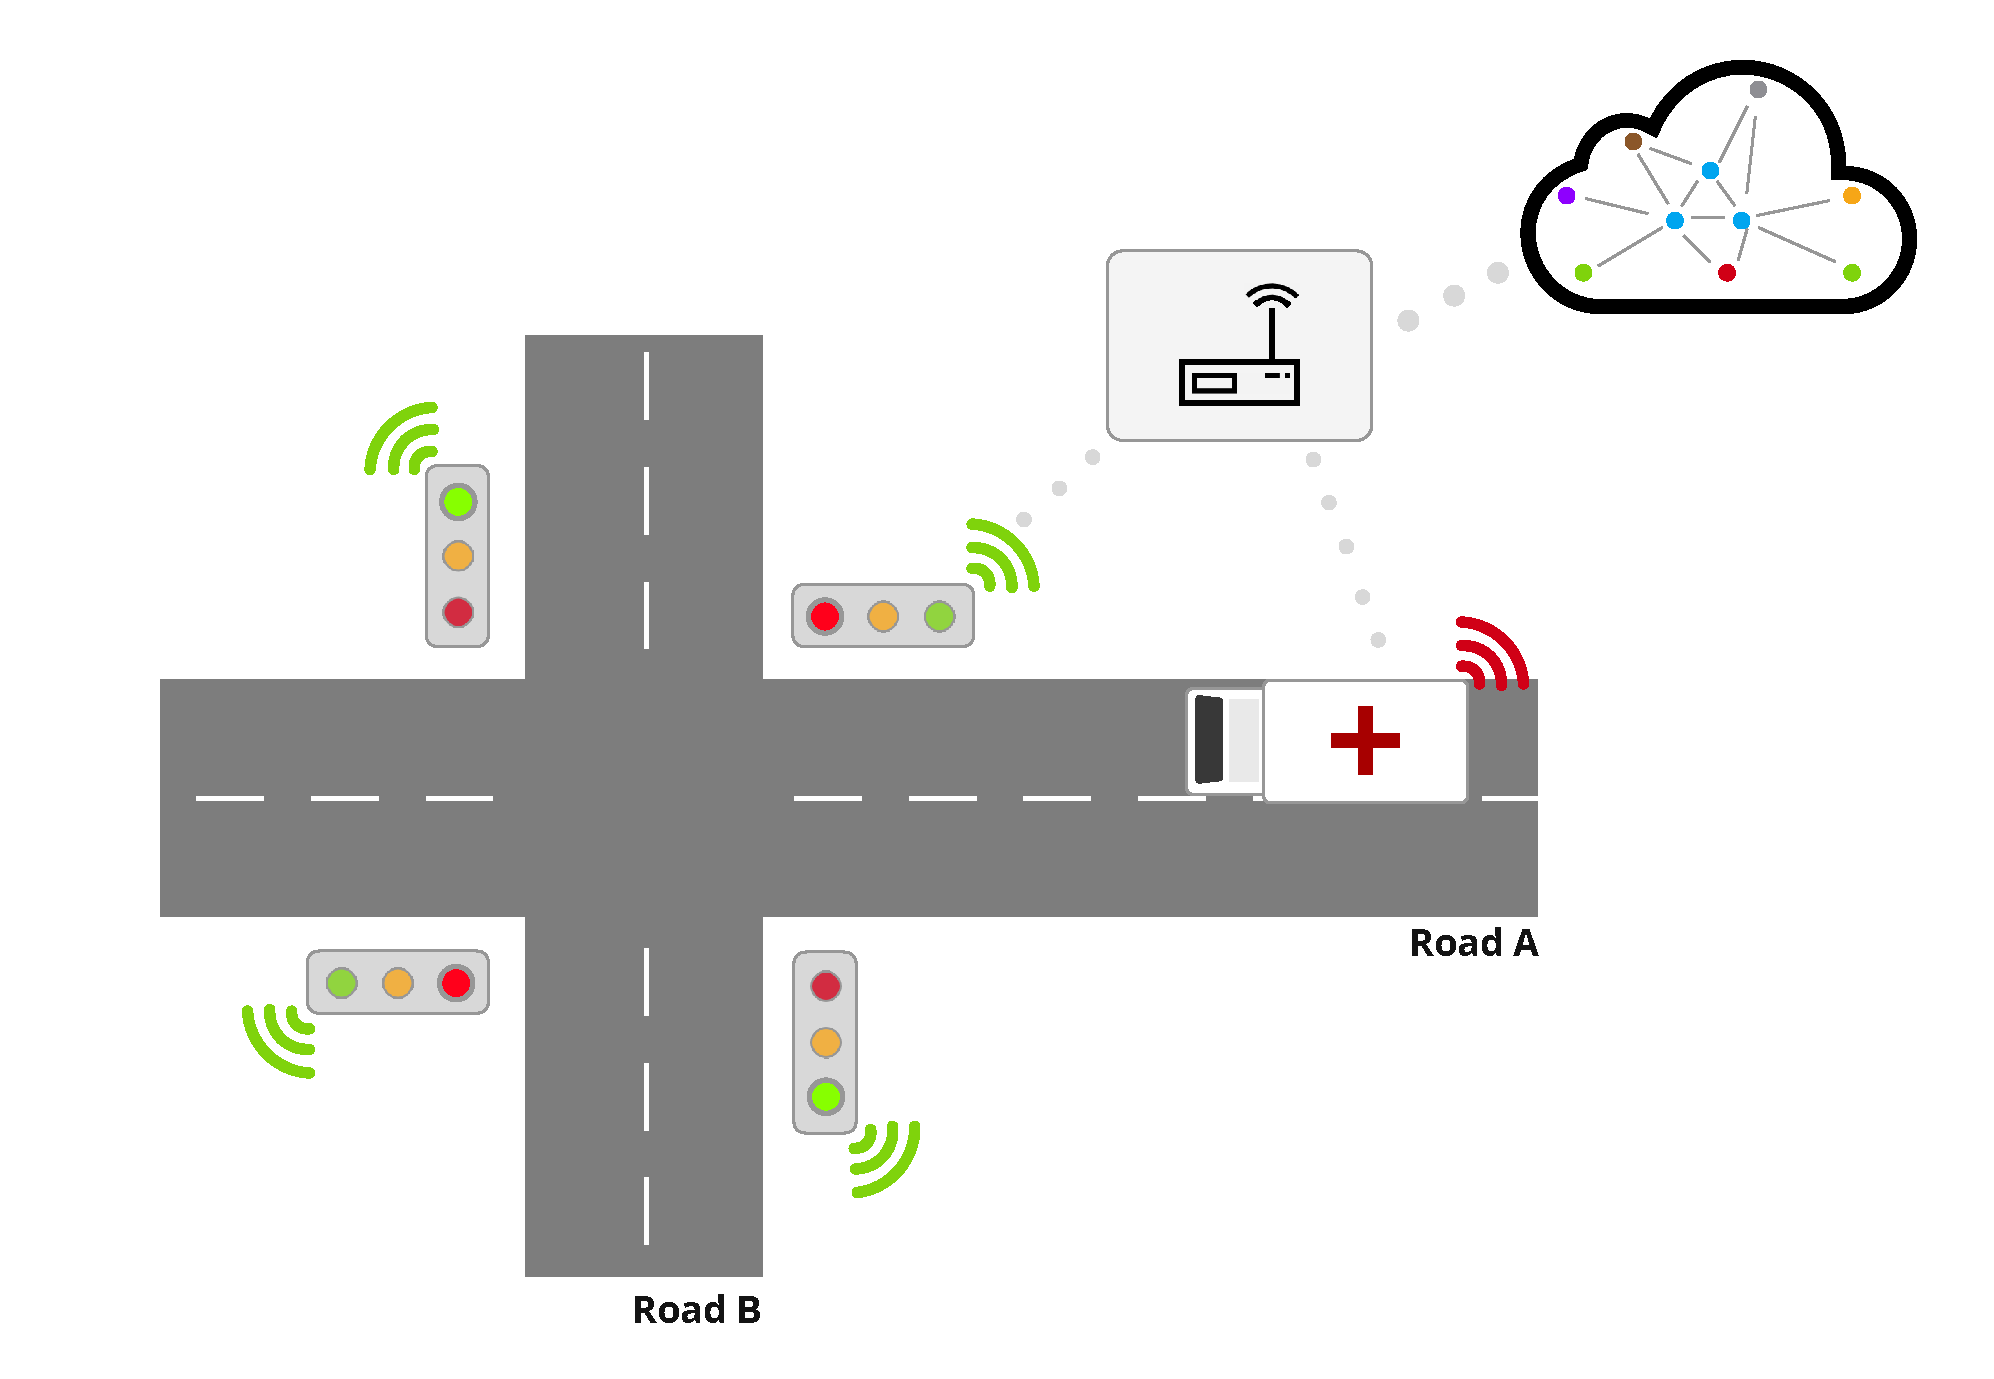
\includegraphics[width=3.5in]{Figures/CrossRoadModel_V1.eps}
\caption{Use case illustration}
\label{fig:CrossRoadModel.eps}
\end{figure}

In order to be as close as possible to a real urban traffic light,
	we prototyped the closest Testbed of a crossroad in Paris.
We took an actual crossing point with its dimension and static timers.
Fig.
\ref{fig:CrossRoadModel.eps} shows IoT interconnection of four traffic lights,
	high priority vehicles and roads.
Our system is described by one intersection (or crossing) of two roads A and B,
	with two traffic lights by road.
The signs and roads can use heterogeneous technologies as presented with different colors.

The roads are connected to the Internet through sensors,
	which are able to detect the arrival of high priority vehicles.
The detection is performed by Touch sensors driven by WSN nodes.
Note that signals on each road should always have different colors (or states).
Of course,
	when the road A traffic light is on green,
	the state of the traffic light on the opposite road,
	must be on red and vice versa.
To access the Internet,
	all messages sent by those objects will go through a Border Router (BR) device and a Middleware or Edge computer.
The Middleware is connected to the Internet and forwards all packets to a Cloud.
Therefore,
	the collected data in the Cloud allow a Middleware to decide for the future state of lights.
Then,
	BR disseminates this decision through the network to the actuators.


%For simplicity, we consider only one priority vehicle coming to a crossing with no other vehicles on the road. Situations like multiple priority vehicles or even crowded roads will not be treated in this work.

%
%In order to match as close as possible real urban traffic light, we made the closest representation of a crossroad in Paris. We took an actual crossing with its dimension and timers. We modeled our solution with a scale of 1:68.
% Make a model

%/ How traffic lights work => simple system
%It works as a simple traffic light system, where signals on each road will have opposite colors (or state). When the road A light is green, the opposite road, its state must be red and vice versa. 
%%
%the will go to green after a 5 seconds extra delay. This extra delay is made to avoid any synchronization problem that could occur.

%[Explanation for this figure how it works => don't worry if some ideas are said again from introduction]




%Fig. \ref{fig:CrossRoadModel.eps} shows IoT interconnection of four traffic lights, priority vehicle and roads. These objects could use heterogeneous technologies as presented with different colors.
%To access the Internet, all messages sent by those objects will pass through a Border Router (BR) device and middleware.
%The middleware would be connected to the Internet and will forward all packets.
%The Cloud would collect and treat those messages and send responses to roads and traffic lights via the same wireless technology.

\subsection{Design Model}

% What is UPPAAL and what can we do with it
Our design is based on UPPAAL model checker software.
It specifies a graph of states with clocks and data variables.
It allows us to model how our system works and simulates all possible traffic lights states.
The modelling allows us to cover all possible cases of lights change of our IoT-UTLC.
It is also a tool for verifying formally the consistancy of traffic light changes:
	GREEN to YELLOW states,
	YELLOW to RED states and RED to GREEN states.
We simulated our system by three automata shown in Fig.
\ref{fig:MiddlewareModel.eps},
	Fig.
\ref{fig:TrafficlightModel.eps} and Fig.
\ref{fig:CloudModel.eps} and available at (https://github.com/IoT-UTLC/Resources).
We proved that our model worked without deadlock and starvation.
It means that in our system,
	there is always a transition to go to the next state.
It proves that the system will not stop functioning over time.
Incoherent situations,
	like four signals on GREEN,
	must not happen.

%Designing this system is important to avoid failures.
%Traffic lights are a safety infrastructure,
%	some behavior like four signals at green should not occur,
%	we have to set rules and model our system to list the dangerous states and avoid them.
%The goal of avoiding deadlock was reached getting a functional system to work with.

% Figure
%\Figure{!htb}{1}{TrafficlightModel.png}{Model of our Traffic Lights in UPPAAL}


\begin{figure*}[!htb]
\centerline{\includegraphics[width=4.5in]{Figures/TrafficlightModel.eps}}
\caption{Model of our Traffic Lights in UPPAAL}
\label{fig:TrafficlightModel.eps}
\end{figure*}

\begin{figure*}[htbp]
\centering
\centerline{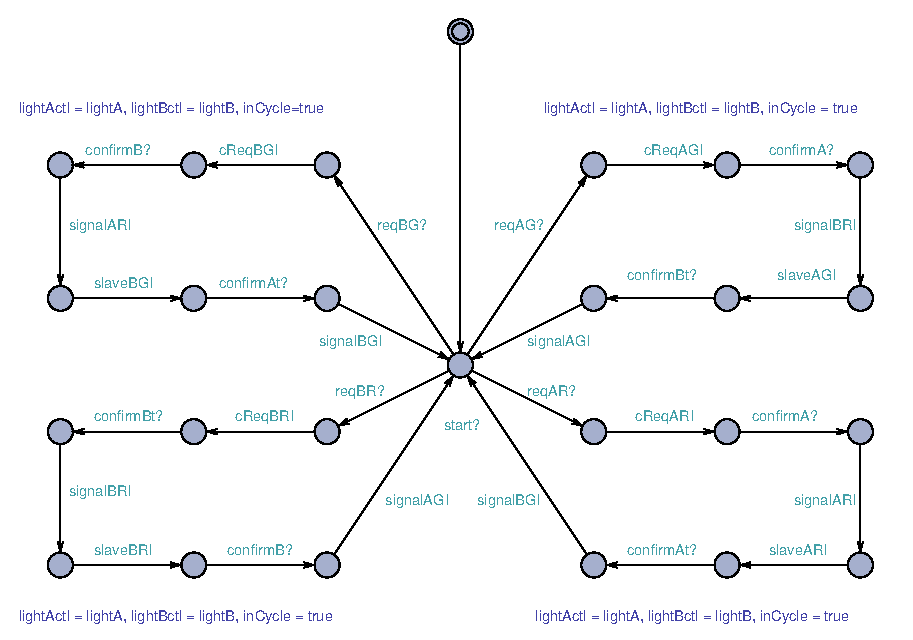
\includegraphics[width=4in]{Figures/MiddlewareModel.eps}}
\caption{Model of our Middleware in UPPAAL}
\label{fig:MiddlewareModel.eps}
\end{figure*}

Fig.
\ref{fig:TrafficlightModel.eps} highlights the model of traffic lights and describes their behavior.
The change of light's state is based on requests and confirmation exchange between lights and the Middleware.
We defined two roles for the traffic lights:
	one is set to master mode and the second one is set to slave mode.
Masters send requests every 60 seconds to change their states while considering the current ones.
Line 6 of Algorithm \ref{Alg:traffic} shows the condition when a light should change its state.
CLK state represents clock or time progress.
\emph{reqAG} and \emph{reqAR} are respectively the requests to ask for GREEN and RED states on road A.
The same is specified for the road B.
When it receives a confirmation from the Middleware,
	a cycle is started to send the signal with the desired state.
Every 30 seconds,
	the traffic lights can change their states,
	starting with GREEN light and then to YELLOW light for 3 seconds after that switching to RED.
They can also start from RED and then change to GREEN state after additional 3 seconds.
We add this extra delay to avoid a dangerous situation when a GREEN state is on the two roads A and B at the same time.
Even if we have messages lost due to the wireless nature of the network,
	our UPPAAL models ensure that this situation doesn't arise.
It has been introduced after experiencing a latency between the WSN and the Cloud platform (see section \ref{sec:Results}).
When GREEN or RED states are actuated,
	confirmation messages are sent to the Middleware.
The pseudo Algorithm \ref{Alg:traffic} summarizes this mechanism.

\RestyleAlgo{algoruled}
\LinesNumbered \begin{algorithm}[ht] \caption{Traffic light\label{Alg:traffic}}
init\_60s\_timer();
	\While{true}{ \If{ end\_timer()}{ send\_request\_new\_state(); \\
	reset\_timer();
	}
\If{msg\_received\_red() and my\_state is green}{ change\_state(yellow);\\
	wait(); \\
	change\_state(red); \\
	send\_confirmation\_to\_middleware();
	}
\If{msg\_received\_green() and my\_state is red}{ change\_state(green);\\
	send\_confirmation\_to\_middleware();
	}
}
\end{algorithm}

The model in Fig.
\ref{fig:MiddlewareModel.eps} defines the different possibilities in terms of internal cycles depending on the request made by traffic lights (\emph{reqAG},
	\emph{reqBG},
	\emph{reqAR} \emph{reqBR}).
Mainly,
	the Middleware sends the message to the Cloud and waits for its response.
Then,
	it sends messages to traffic lights master and slave to change their state following this order:
	every light go to RED before setting GREEN signals.
It also uses acknowledgments from the traffic lights to ensure that the new state has been set.
In order to ensure these two features,
	we used a system to retain messages if the IoT Cloud Platform send GREEN states before RED states (see line 3 of Algorithm.
\ref{Alg:conf} ).
Algorithm \ref{Alg:conf} shows a simple description showing how the Middleware confirms the order of traffic lights changes.


% By subscription,
% 	the middleware gets new states for the traffic lights and sends them accordingly to the master and slave traffic lights.
% It sends red states first and then green states to avoid unwanted behaviors.
% It also uses acknowledgments from the traffic lights to ensure that the new state has been set.
% In order to ensure these two features,
% 	we used a system to retain messages if the IoT Cloud Platform send green states before red states.
% Algorithm \ref{Alg:conf} shows how it works.

\RestyleAlgo{algoruled}
\LinesNumbered \begin{algorithm}[ht] \caption{Middleware confirmation\label{Alg:conf}}
\If{message\_received()}{ \If{ is\_green()}{ retain\_msg();
	//green then red }
\Else{ \If { retained\_msg\_exist()}{ update\_to\_red();
	//green then red }\Else{ update\_to\_red();
	//red then green }}
}
\While{true}{ confirmation\_red\_lights(); \\
	update\_to\_green(); \\
	confirmation\_green\_lights();
	}
\end{algorithm}
\begin{figure}[!htb]
\centering
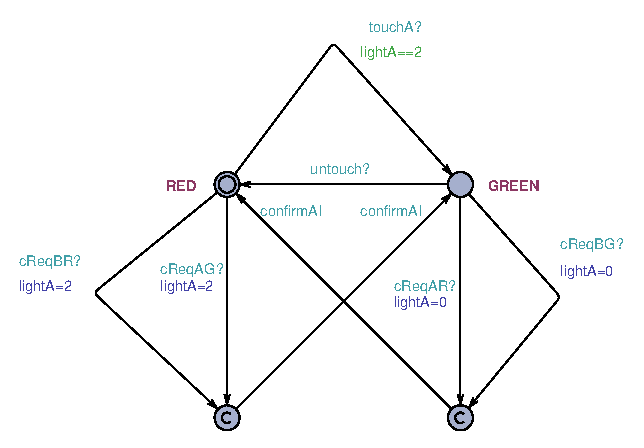
\includegraphics[width=3.2in]{Figures/CloudModel.eps}
\caption{Model of our Cloud variables in UPPAAL}
\label{fig:CloudModel.eps}
\end{figure}


We introduced the IoT Cloud Platform model shown in Fig.
\ref{fig:CloudModel.eps}.
It simulates the subscription mechanism according to messages sent by the Middleware to update collected data.
We defined two states RED and GREEN without a transition state like YELLOW state defined for the traffic lights.
The condition \emph{touchA} indicates if the road A detects the high priority vehicle.
The name \emph{touch} is related to the type of sensor integrated in our prototype (see next section).
The Cloud confirms to the Middleware that the state is changed by sending a message \emph{confirmA}.

Exchanged messages within our WSN are based on IEEE 802.15.4 stack.
And our Middleware defines QoS levels of exchanged messages via MQTT protocol.
